\section*{Results}

\begin{figure}[H]
  \centering
  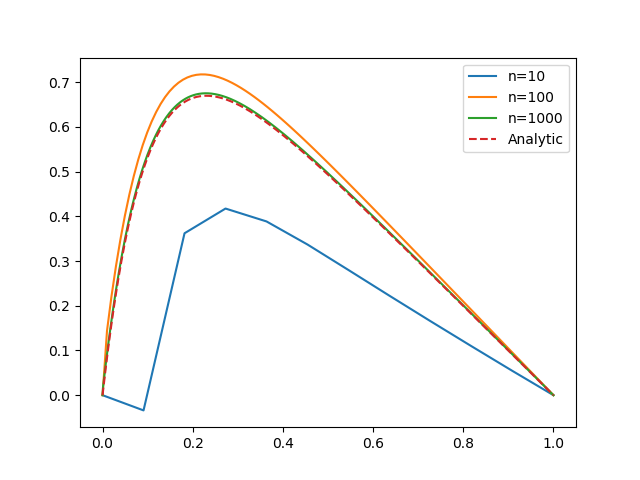
\includegraphics[width=0.66\textwidth]{../figures/thomas.png}
  \caption{Comparison of analytic solution and numerical approximations}
  \label{fig:a}
\end{figure}


\begin{table}[htp]
  \centering
  \csvautotabular{../data/relative_error.csv}
  \caption{Maximum relative error between analytic and numeric solution.}
  \label{table:relative_error}
\end{table}



After running the thomas and toeplitz algorithm on matrixes from 10x10 to
1000000 x 1000000, and the lower/upper decomposition + backward subtitution (LU)
on matrixes from 10x10 to 1000x1000 ten times and taking the average we got the
results in \cref{table:normalized}.

\begin{table}[htp]
  \centering
  \csvautotabular{../processed_data/algorithm_time.csv}
  \caption{Summary of algorithm times.}
  \label{table:normalized}
\end{table}


To see how the algorithm time for our different methods scales with n we divide
all timings with n (\cref{table:normalized}). Both the thomas and toeplitz
algorithm times (normalized by n) are of the same order, as was expected from
the counting of flops. The times for LU show an increase of to orders of magnitude
for each magnitude increase in n. This is consistent with our expectations
of the LU algorithm time being proportional to $n^3$.

\begin{table}[htp]
  \centering
  \csvautotabular{../processed_data/normalized.csv}
  \caption{Algorithm times divided by n.}
  \label{table:normalized}
\end{table}


Comparing the algorithm times of thomas and toeplitz (\cref{table:comparison})
we see they are the same order of magnitude. Theoretically we would
expect the toeplitz algorithm to be $\frac{9 FLOPS}{4 FLOPS} \approx 2.25$ times as fast as
toeplitz, and our results for larger values of n are quite close.

\begin{table}[htp]
  \centering
  \csvautotabular{../processed_data/comparison.csv}
  \caption{Algorithm times of thomas divided by that of toeplitz.}
  \label{table:comparison}
\end{table}
